% This is samplepaper.tex, a sample chapter demonstrating the
% LLNCS macro package for Springer Computer Science proceedings;
% Version 2.20 of 2017/10/04
%
%\documentclass{scrbook}
\documentclass[runningheads]{llncs}
%
\usepackage{graphicx}
% Used for displaying a sample figure. If possible, figure files should
% be included in EPS format.
%
\usepackage[ngerman]{babel}
% If you use the hyperref package, please uncomment the following line
% to display URLs in blue roman font according to Springer's eBook style:
% \renewcommand\UrlFont{\color{blue}\rmfamily}

\usepackage[T1]{fontenc}
\usepackage{lmodern}
\usepackage{listings}
\usepackage{textcomp}
\usepackage{amsfonts}
\usepackage{amsmath}
\usepackage{hyperref} 
\begin{document}

\title{Vergleich von Feuchtesensoren in Bezug auf Genauigkeit\\Proseminar Mobile Computing
\\03.05.2019}
%\date{3.Mai 2019}

\titlerunning{Vergleich von Feuchtesensoren}
% If the paper title is too long for the running head, you can set
% an abbreviated paper title here
%
\author{Ilia Chupakhin\\Betreuer Jan Formanek}

\authorrunning{Ilia Chupakhin}
% First names are abbreviated in the running head.
% If there are more than two authors, 'et al.' is used.
%


\institute{Karlsruher Institut für Technologie, Kaiserstraße 12, 76131 Karlsruhe, Deutschland
	\\\email{info@kit.edu}
	\\\url{https://www.kit.edu/} 
	\and
Technology for Pervasive Computing (TECO), Vincenz-Prießnitz-Straße 1,76131 Karlsruhe, Deutschland
	\\\email{sekretariat@teco.edu}
	\\\url{https://www.teco.edu/}
}
%
\maketitle              % typeset the header of the contribution
%
\begin{abstract}
Bestimmte Modelle von Feuchtesensoren wurden mit einem Referenzsensor in Bezug auf Genauigkeit verglichen. Der Referenzsensor ist SHT75. Die zu vergleichenden Sensoren sind SHT31, HTU21D, BME280, DHT22. Es waren jeweils vier Exemplare von SHT31, HTU21D, DHT22 und drei Exemplare von BME280 vorhanden. Der Referenzsensor war ein Einzelstück. Die Messungen wurden bei vier unterschiedlichen relativen Luftfeuchtigkeitsniveaus durchgeführt. Die gemessenen Werte wurden mithilfe von statistischen Methoden analysiert und anschließend wurde anhand der untersuchten Stichprobe auf die zu erwartende Genauigkeit der gesamten Population von gegebenen Sensoren geschlossen.    

\keywords{Sensor \and Luftfeuchtigkeit \and Vergleich \and SHT75 \and SHT31 \and HTU21D \and BME280 \and DHT22}
\end{abstract}
%
%
%
\section{Einleitung}
\subsection{Motivation}
Es gibt eine große Auswahl von Feuchtesensoren auf dem Markt. Die wichtigsten Kriterien bei der Wahl eines Sensors sind der Preis und die Messgenauigkeit. Die beiden Kriterien korrelieren miteinander: üblicherweise, je höher der Preis ist, umso höher ist die Messgenauigkeit. Doch manchmal kostet ein Sensor fünf- oder zehnmal so viel wie ein anderer, obwohl laut ihren Datenblättern der teurere nur um ein Prozent präziser die Luftfeuchtigkeit  messen kann als der billigere. Der Preisunterschied wird umso spürbarer, wenn man die Sensoren in großen Mengen braucht. Deshalb will man sich für billigere Sensoren entscheiden, wenn ein solcher Präzisionsunterschied für den beabsichtigten Einsatzzweck nur wenig oder komplett irrelevant ist. Allerdings entspricht die in den Datenblättern angegebene Messgenauigkeit manchmal nicht der tatsächlichen. Darüber hinaus fehlen oft die Angaben über die zu erwartende Streuung von Messwerten. Diese Probleme sind insbesondere bei billigen Sensoren öfter anzutreffen. Deswegen wollte man zuerst eine kleine Menge von Sensoren kaufen und ihre Messgenauigkeit experimentell überprüfen, bevor man die Sensoren in großen Mengen einkauft.  
\subsection{Zielsetzung}
Im Rahmen des Proseminars wird eine Stichprobe von vier unterschiedlichen Modellen der Feuchtesensoren mit einem Referenzsensor in Bezug auf Messgenauigkeit verglichen. Von jedem Modell außer dem Referenzsensor werden mehrere Exemplare untersucht. Die Messungen werden bei vier unterschiedlichen relativen Luftfeuchtigkeitsstufen durchgeführt. Danach werden die gesammelten Daten einer statistischen Analyse unterzogen. Basierend auf der statistischen Analyse wird eins der untersuchten Modelle von Feuchtesensoren gefunden, dessen Messwerte den Messwerten vom Referenzsensor am nächsten liegen.
\subsection{Begriffe und Abkürzungen}
Luftfeuchtigkeitsstufe oder Luftfeuchtigkeitsniveau - relative Luftfeuchtigkeit 50\%, 60\%, 70\% oder 80\%.\\
RH(kommt von \textbf{r}elative \textbf{h}umidity) - relative Luftfeuchtigkeit.\\
Mit Luftfeuchtigkeit wird die relative Luftfeuchtigkeit gemeint.\\
Mit Sensor wird Feuchtesensor gemeint.\\
Mit Testsensor wird einer der mit dem Referenzsensor zu vergleichenden Sensoren gemeint, also HTU21D, SHT31, BME280 oder DHT22.\\
\section{Vorbereitung auf das Messexperiment}Bevor das Messexperiment durchgeführt werden konnte, mussten die dafür benötigten Soft- und Hardwarekomponenten erstellt beziehungsweise zusammengesetzt werden. Außerdem musste eine passende experimentelle Umgebung eingerichtet werden.
\subsection{Hardware}
Die Datenblätter für die benutzten Hardware-Elemente sind im Literaturverzeichnis verlinkt.\\
Referenzsensor: SHT75
\\Die zu vergleichenden Sensoren: SHT31, HTU21D, BME280, DHT22
\\Mikrocontroller: NodeMCU ESP32
\\SD-Speicherkartenmodul: Pollin
\\SD-Speicherkarte: Kingston 16GB
\\Lochrasterplatine, Kabel, Buchsenleisten
\\Micro-USB Kabel und Laptop
\\\\Die Buchsenleisten wurden auf die Lochrasterplatine gelötet und verkabelt. Alle Sensoren, der Mikrocontroller und das SD-Speicherkartenmodul wurden in die Buchsenleisten eingesteckt. Die SD-Speicherkarte wurde in das SD-Speicherkartenmodul eingelegt. Der Mikrocontroller wurde über ein Micro-USB-Kabel zum Laptop angeschlossen. Siehe die Abbildung 1.

\begin{figure}[h]
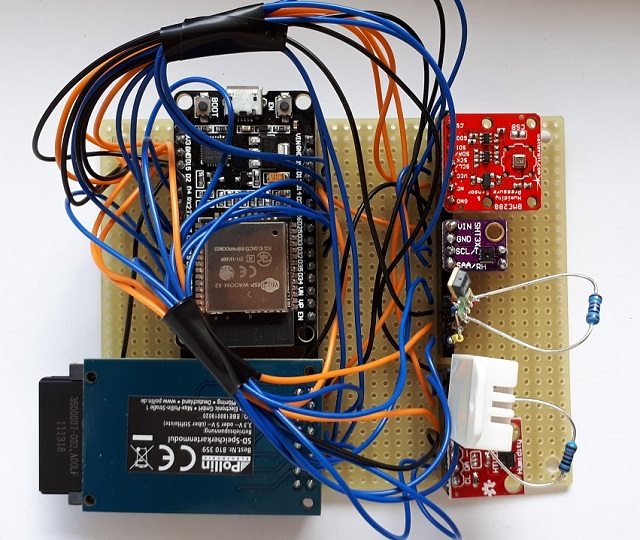
\includegraphics[width=\textwidth]{pictures/platine.jpg}
\caption{Platine mit Sensoren}
% \label{fig1}
\end{figure}
     
\subsection{Software}
Zum Steuern der Hardware-Elementen wurde ein Programm in der Entwicklungsumgebung Arduino (Version 1.8.9)  geschrieben. Das Programm ist im Anhang zu finden. Zum Datenaustausch wurde der I\textsuperscript{2}C-Datenbus benutzt. Für alle Sensoren sowie für den Mikrocontroller mussten noch zusätzlich externe Bibliotheken installiert werden. Bei manchen der installierten Bibliotheken war es nicht vorgesehen, dass man die PIN-Nummern für serial clock und serial data Kanäle nach seiner Wahl eingeben kann. Diese Funktionalität war aber notwendig, weil mehrere Sensoren zu einem Mikrocontroller angeschlossen werden mussten. Deswegen wurden folgende Funktionen zusätzlich zu den bereits vorhandenen implementiert:
\begin{itemize}
\item In der Datei Adafruit\textunderscore SHT31.h:
\end{itemize}
\begin{lstlisting}[
  % one can adjust spacing here if required
  % aboveskip=2.5\baselineskip,
  % belowskip=-.8\baselineskip,
  %caption={Example Java Listing},
  %label=L1,
  language=C,
  %float
  ]
boolean begin(int sda, int scl, uint8_t i2caddr = SHT31_DEFAULT_ADDR);
\end{lstlisting}
\begin{itemize}
\item In der Datei Adafruit\textunderscore SHT31.cpp:
\end{itemize}
\begin{lstlisting}[language=C]
boolean Adafruit_SHT31::begin(int sda, int scl, uint8_t i2caddr) {
  Wire.begin(sda, scl);
  _i2caddr = i2caddr;
  reset();
  return true;
}
\end{lstlisting}
\begin{itemize}
\item In der Datei Adafruit\textunderscore HTU21DF.h:
\end{itemize}
\begin{lstlisting}[language=C]
boolean begin(int sda, int scl);
\end{lstlisting}
\begin{itemize}
\item In der Datei Adafruit\textunderscore HTU21DF.cpp:
\end{itemize}
\begin{lstlisting}[language=C]
boolean Adafruit_HTU21DF::begin(int sda, int scl) {
  Wire.begin(sda,scl);
  reset();
  Wire.beginTransmission(HTU21DF_I2CADDR);
  Wire.write(HTU21DF_READREG);
  Wire.endTransmission();
  Wire.requestFrom(HTU21DF_I2CADDR, 1);
  return (Wire.read() == 0x2); // after reset should be 0x2
}
\end{lstlisting}
Das geschriebene Programm funktioniert folgendermaßen:\\ Nach dem Einschalten des Mikrocontrollers wird eine neue Textdatei auf der SD-Speicherkarte einmal erstellt. Die Temperatur- und Luftfeuchtigkeitswerte werden von allen Sensoren einmal pro Sekunde ausgelesen. Die Werte werden temporär auf dem Mikrocontroller gespeichert. Nach zehn Auslesezyklen werden die gespeicherten Werte in die erstellte Textdatei hingeschrieben. Danach wird das Programm wie vorher abgearbeitet.
\subsection{Messaufbau und Umgebung für das Messexperiment}
Das Messexperiment wurde in einem Zimmer mit der Luftfeuchtigkeit 48-52\% bei der Temperatur 27-31$^\circ$C durchgeführt. Die Platine mit Sensoren wurde in einer Plastikkiste an die Wand befestigt. In der Kiste wurde eine Metallschüssel mit einem feuchten Tuch und Schwamm platziert. Siehe die Abbildung 2.  
\begin{figure}[h]
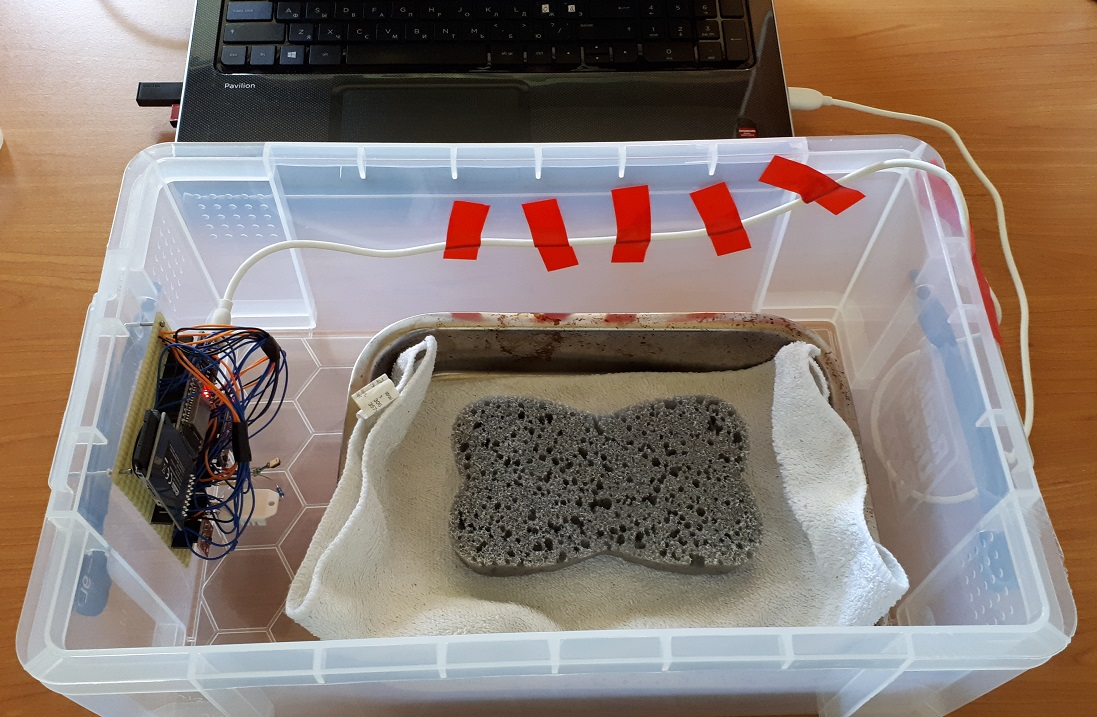
\includegraphics[width=\textwidth]{pictures/messaufbau.jpg}
\caption{Messaufbau}
% \label{fig1}
\end{figure}
\section{Durchführung des Messexperimentes}
\subsection{Planung des Messexperimentes}
Die Messung wird bei jeweils 50, 60, 70 und 80\% RH durchgeführt. Die Messwerte werden einmal pro Sekunde ausgelesen. Für jede der vier Luftfeuchtigkeitsstufen werden 170 Messzyklen durchgeführt. Die Messung startet bei 50\% RH. Während des Messexperimentes wird die relative Luftfeuchtigkeit stufenweise bis 80\% erhöht und anschließend wieder bis 50\% gesenkt. Das Messexperiment wird für jedes Exemplar von Testsensoren durchgeführt.
\subsection{Vernachlässigungen und Anmerkungen}
\begin{itemize}
\item Aufgrund von Einschränkungen der experimentellen Umgebung und des Messaufbaues darf die Luftfeuchtigkeit in der experimentellen Umgebung im Bereich $\pm$2\% von der gewünschten schwanken und wird somit als konstant betrachtet.
\end{itemize}
\begin{itemize}
\item Um die Luftfeuchtigkeit in der Plastikkiste während der Messung konstant zu halten, wird der Kistendeckel manipuliert.
\end{itemize}
\begin{itemize}
\item Die Sensoren besitzen unterschiedliche Antwortzeiten. Laut den Datenblättern sind die Antwortzeiten: 8 Sekunden für SHT75, 10 Sekunden für HTU21D, 8 Sekunden für SHT31, 1 Sekunde für BME280, nicht angegeben für DHT22. Damit die Antwortzeiten möglichst kleine  Auswirkung auf die Messergebnisse haben, wird nach dem Wechseln zu der nächsten Luftfeuchtigkeitsstufe zwei Minuten gewartet, bis die nächste Messung startet.
\end{itemize}
\begin{itemize}
\item Die einzelnen Sensoren werden nicht parallel, sondern nacheinander vom Mikrocontroller angesprochen. Trotzdem wird angenommen, dass die Luftfeuchtigkeitswerte von allen fünf Sensoren zum gleichen Zeitpunkt ausgelesen werden, weil das Auslesen aller Sensoren insgesamt weniger als 200 Millisekunden dauert und in der experimentellen Umgebung sind jegliche Änderungen der Luftfeuchtigkeit innerhalb so einer kurzen Zeitspanne vernachlässigbar.
\end{itemize}
\begin{itemize}
\item Aus Kostengründen war die Stichprobe relativ klein. Es waren ein Exemplar von dem Referenzsensor, drei Exemplare von BME280 und jeweils vier Exemplare von den anderen Sensoren vorhanden. Die Größe der Stichprobe spiegelt sich in der Breite des Konfidenzintervalles wider.\footnote[1]{Siehe das Kapitel Auswertung der Messergebnisse}
\end{itemize}
\begin{itemize}
\item Die Messung bei der steigenden und anschließend bei der senkenden Luftfeuchtigkeit war notwendig, um die Hysterese von Sensoren herauszufinden. Das heißt, die Messewerte bei derselben  Luftfeuchtigkeit können unterschiedlich ausfallen abhängig davon, ob die Luftfeuchtigkeit vor der Messung gestiegen oder gesunken ist.     
\end{itemize}
\subsection{Ablauf des Messexperimentes}
Die relative Luftfeuchtigkeit im Zimmer wurde im Bereich 48-52\% während des gesamten Messexperimentes konstant gehalten. Die Plastikkiste wurde auf den Tisch nahe des Laptops gestellt. Die ersten Exemplare von den Testsensoren wurden angeschlossen. Der Mikrocontroller wurde zum Laptop angeschlossen. Die Messwerte waren auf dem Bildschirm zu sehen und wurden einmal pro Sekunde aktualisiert. Die Messung bei der Luftfeuchtigkeit 50\% wurde durchgeführt. Danach wurde die Metallschüssel mit einem feuchten Tuch und Schwamm in die Plastikkiste eingelegt. Die Luftfeuchtigkeit in der Kiste ist auf 60\% gestiegen. Die Messung bei der Luftfeuchtigkeit 60\% wurde durchgeführt. Danach wurde der Deckel auf die Kiste gelegt, so dass sie etwa zu 2/3 abgedeckt war. Die relative Luftfeuchtigkeit in der Kiste ist auf 70\% gestiegen. Die Messung bei der Luftfeuchtigkeit 70\% wurde durchgeführt. Danach wurde die Kiste mit dem Deckel komplett abgedeckt. Die Luftfeuchtigkeit in der Kiste ist auf 80\% gestiegen. Die Messung bei der Luftfeuchtigkeit 80\% wurde durchgeführt. Anschließend wurden analog die Messungen bei der absteigenden Luftfeuchtigkeit durchgeführt. Das Messexperiment wurde für alle Exemplare von Testsensoren durchgeführt (insgesamt vier Mal).

\section{Auswertung der Messergebnisse}
Nachdem das Messexperiment abgeschlossen war, mussten die Messergebnisse mithilfe von statistischen Methoden ausgewertet werden. Die Textdateien mit den Messdaten wurden im Programm Apache OpenOffice Calc bearbeitet.
\\Zuerst wurden die Messdaten manuell gefiltert. Die Messungen während den Übergängen zwischen Luftfeuchtigkeitsstufen wurden entfernt. Auch die Messungen in den nächsten zwei Minuten nach dem Übergang mussten entfernt werden, um den Einfluss von unterschiedlichen Antwortzeiten der Sensoren auf die statistische Auswertung zu reduzieren. Während der Messung kam es manchmal zu den leichten Überschreitungen von den vereinbarten Grenzen von $\pm$2\% RH. Diese Daten wurden ebenso aus den zu analysierenden Messdaten entfernt.
\\Danach wurde in jeder Messung und für jeden Sensor die Abweichung von den Referenzwerten ausgerechnet.
\begin{equation}
A=\varphi_{\text{ref}} - \varphi
\label{formel1}
\end{equation}
$A$ - Abweichung, $\varphi_{\text{ref}}$ - relative Luftfeuchtigkeit gemessen von dem Referenzsensor, $\varphi$ - relative Luftfeuchtigkeit gemessen von einem Testsensor.
\\Die Abbildungen drei bis sechs sind Streudiagramme, die die Abweichungen der Messwerte von den Referenzwerten während der Messung bei 50\% RH zeigen. Die Streudiagramme für die Messungen bei den anderen Luftfeuchtigkeitsstufen sind im Anhang zu finden. Zur Erinnerung, die Messwerte wurden einmal pro Sekunde ausgelesen und für jede Luftfeuchtigkeitsstufe wurden 170 Messwerte analysiert. An der Stelle sollte es angemerkt werden, dass die Kurven auf den Streudiagrammen für die Messungen bei 50 und 80\% RH glatter als für die Messungen bei 60 und 70\% RH sind. Das liegt daran, dass während der Messungen bei 60 und 70\% RH die Luftfeuchtigkeit stärker schwankte als bei 50 und 80\% RH. Der Kistendeckel musste oft hin- und hergeschoben werden, damit die Luftfeuchtigkeit im Bereich 60$\pm$2\%RH beziehungsweise 70$\pm$2\%RH bleibt. Da die Sensoren unterschiedliche Antwortzeiten haben, schwankten auch die Abweichungen zwischen den einzelnen Messungen stärker als während der Messungen bei 50\% und 80\% RH. 

\begin{figure}[h]
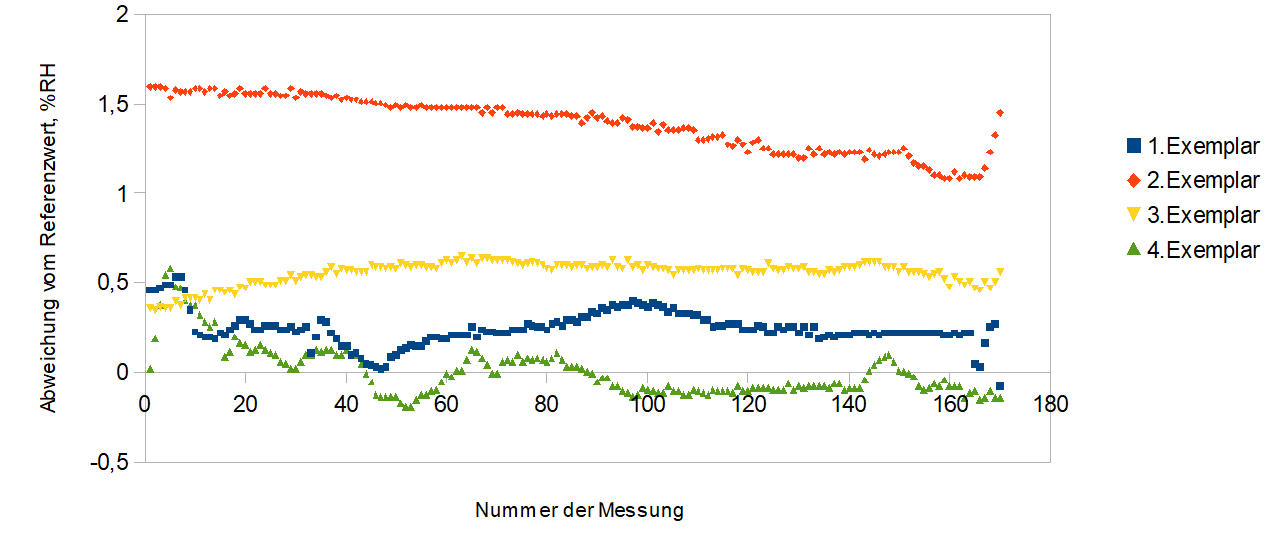
\includegraphics[width=\textwidth]{pictures/HTU21D_50.png}
\caption{HTU21DF Abweichung von Referenzwerten während der Messung bei 50\% RH}
% \label{fig1}
\end{figure}

\begin{figure}[h]
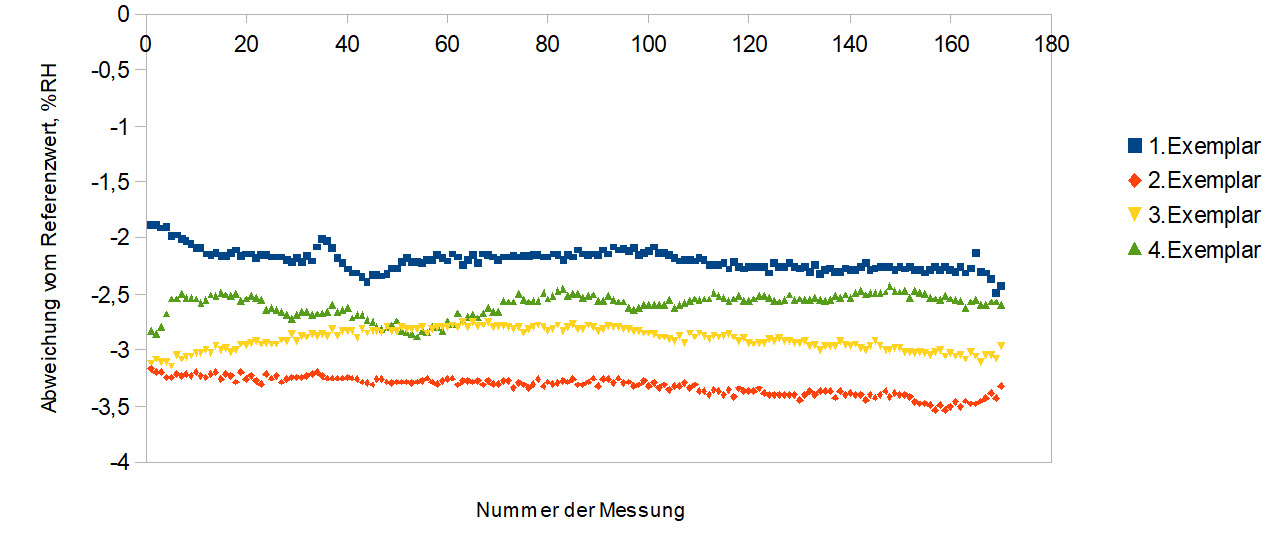
\includegraphics[width=\textwidth]{pictures/SHT31_50.png}
\caption{SHT31 Abweichung von Referenzwerten während der Messung bei 50\% RH}
% \label{fig1}
\end{figure}


\begin{figure}[h]
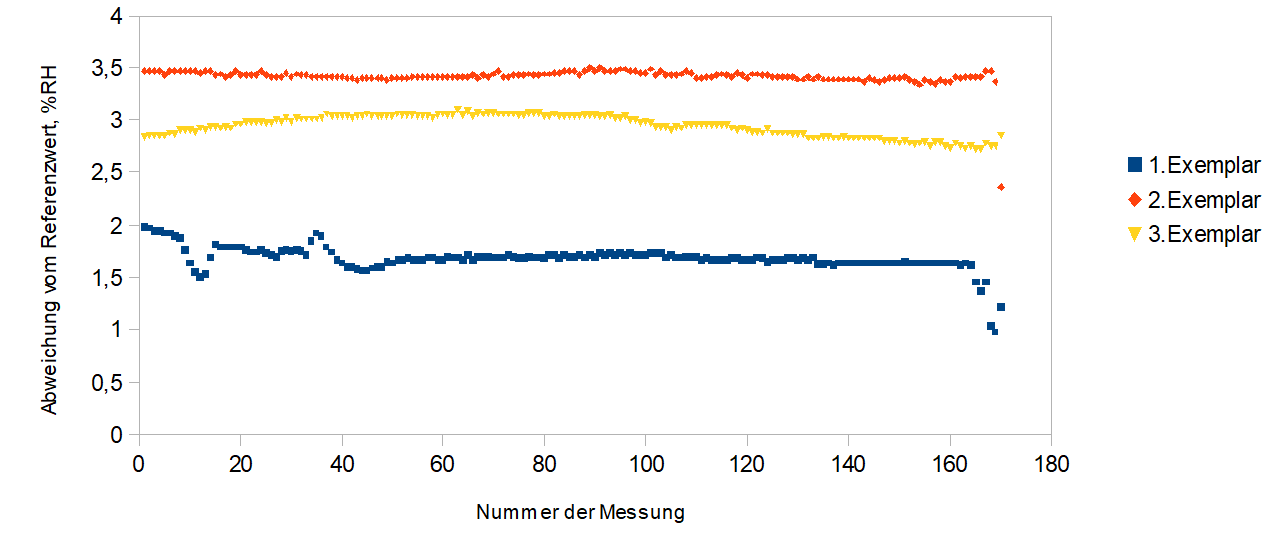
\includegraphics[width=\textwidth]{pictures/BME280_50.png}
\caption{BME280 Abweichung von Referenzwerten während der Messung bei 50\% RH}
% \label{fig1}
\end{figure}

\begin{figure}[h]
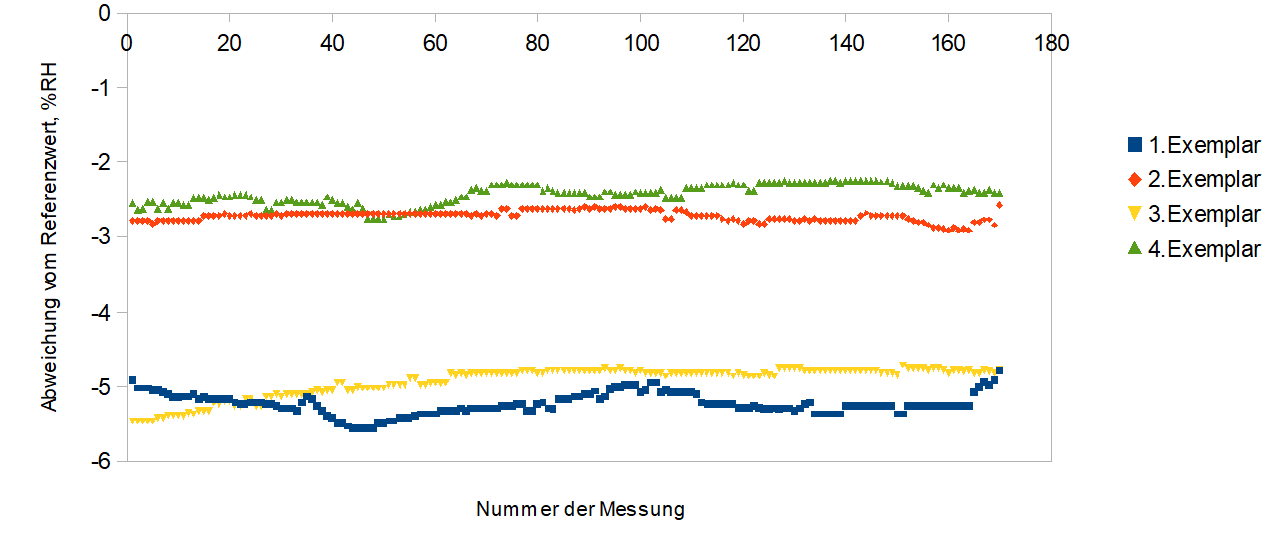
\includegraphics[width=\textwidth]{pictures/DHT22_50.png}
\caption{DHT22 Abweichung von Referenzwerten während der Messung bei 50\% RH}
% \label{fig1}
\end{figure}

Anschließend wurde für jedes Exemplar der Testsensoren und für jede Luftfeuchtigkeitsstufe die absolute durchschnittliche Abweichung von den Referenzwerten ausgerechnet.
\begin{equation}
\overline{A}=\frac{1}{170}\cdot\sum_{i=1}^{170}|A_{i}| 
\label{formel2}
\end{equation}
%$i$ - Nummer der Messung.
%TODO Formel abs Varianz 
\\Absolute durchschnittliche Abweichung bedeutet, dass es irrelevant ist, ob zum Beispiel der gemessene Wert um 3\% RH größer oder kleiner als der Referenzwert ist. Wichtig ist nur, dass er um drei Prozent von dem Referenzwert abweicht. Die Motivation hinter der Entscheidung, einen absoluten Wert auszurechnen statt auf das Vorzeichen zu achten, wird am Besten durch ein kleines Gegenbeispiel ersichtlich sein: bei der ersten Messung betrage die Abweichung +5\% RH und bei der zweiten -6\% RH. Die durchschnittliche Abweichung wäre also $(5+(-6))/2=0.5$. Dann würde man sich denken, dass der Sensor nur eine kleine Abweichung von den Referenzwerten hat, obwohl es nicht stimmt.
\\Nachdem die Messwerte für die einzelnen Exemplare von Sensoren analysiert wurden, konnte man mit der Analyse der gesamten Stichprobe anfangen und anschließend Aussagen über die gesamte Population von Sensoren treffen. Allerdings war die Stichprobe relativ klein (drei bis vier Exemplare von Testsensoren). Auch die Angaben über die Varianz der gesamten Population haben gefehlt. Eine Lösung des Problems besteht darin, dass man die unbekannte Populationsvarianz durch die Stichprobenvarianz ersetzt und zum Ausrechnen der Konfidenzintervalle die Koeffizienten für die t-Verteilung (auch als Studentsche Verteilung bekannt) nimmt, die auch von der Größe der Stichprobe abhängig sind.  
\\Zuerst wurden für jedes Modell der Sensoren der Mittelwert und die Varianz von der absoluten mittleren Abweichung ausgerechnet und zwar für jede Luftfeuchtigkeitsstufe separat. Die Hysterese ist in die Rechnung mit einbezogen, denn es wurden die absoluten mittleren Abweichungen beim Anstieg und beim Abstieg RH für jede Luftfeuchtigkeitsstufe genommen.

\begin{equation}
\mu=\frac{1}{m}\cdot\sum_{i=1}^{m}\overline{A}_{i}
\label{formel3}
\end{equation}

\begin{equation}
\sigma^2=\frac{1}{m-1}\cdot\sum_{i=1}^{m}(\mu-\overline{A}_{i})^2
\label{formel4}
\end{equation}

\begin{center}
$
m = \begin{cases}
    2 \cdot j & \text{ falls die Luftfeuchtigkeitsstufe} \neq 80\% \\j  & \text{sonst}
\end{cases}
$
\end{center}
$j$ - Stichprobengröße, $\mu$ - Mittelwert, $\sigma^2$ - Varianz\\
Dann wurde der Standardfehler des Mittelwertes ausgerechnet.
\begin{equation}
SEM=\frac{\sigma}{\sqrt{j}}
\label{formel5}
\end{equation}
Mit den ausgerechneten Werten konnte man schließlich die Konfidenzintervalle bestimmen. Da die Stichprobe relativ klein war, hat man sich für die 90\%-Konfidenzintervalle statt der typischen 95\%-Konfidenzintervalle entschieden.
\begin{equation}
K=[\kappa_{\text{min}};\kappa_{\text{max}}]=[\mu-t\cdot SEM;\mu+t\cdot SEM]
\label{formel6}
\end{equation}
$t$ ist der t-Koeffizient aus der Tabelle für die gegebene Stichprobengröße.\\        
Auch die durchschnittliche Hysterese wurde ausgerechnet.
\begin{equation}
\overline{H}=\frac{1}{j}\cdot\sum_{i=1}^{j}|\overline{A}_{\text{Anstieg}}-\overline{A}_{\text{Abstieg}}|
\label{formel7}
\end{equation}
$j$ - Stichprobengröße, $\overline{A}_{\text{Anstieg}}$ und $\overline{A}_{\text{Abstieg}}$ - durchschnittliche absolute Abweichung bei steigender beziehungsweise sinkender Luftfeuchtigkeit.\\
In den Tabellen 1 - 5 sind die ausgerechneten Werte zu sehen.

\begin{table}[!h]
\centering
\caption{HTU21D Stichprobenanalyse, \% RH}
\label{tab:my-table}
\resizebox{\textwidth}{!}{%
\begin{tabular}{|c|c|c|c|c|c|c|}
\hline
Luftf. & Mittelwert & Varianz & Std.fehler des Mit.wert. & Hysterese & Konf.intervall Min & Konf.intervall Max \\ \hline
50\%             & 0,4742     & 0,1617  & 0,2011                          & 0,3448                      & 0,0010                                & 0,9473                               \\ \hline
60\%             & 1,2861     & 0,4154  & 0,3223                          & 0,9903                      & 0,5278                                & 2,0444                               \\ \hline
70\%             & 0,8166     & 0,2559  & 0,2529                          & 0,2634                      & 0,2214                                & 1,4117                               \\ \hline
80\%             & 0,9750     & 0,5393  & 0,3672                          &                             & 0,1111                                & 1,8390                               \\ \hline
\end{tabular}%
}
\end{table}

\begin{table}[!h]
\centering
\caption{SHT31 Stichprobenanalyse, \% RH}
\label{tab:my-table}
\resizebox{\textwidth}{!}{%
\begin{tabular}{|c|c|c|c|c|c|c|}
\hline
Luftf. & Mittelwert & Varianz & Std.fehler des Mit.wert. & Hysterese & Konf.intervall Min & Konf.intervall Max \\ \hline
50\%             & 3,0389     & 0,3625  & 0,3010                          & 0,5717                      & 2,3306                                & 3,7472                               \\ \hline
60\%             & 2,9858     & 0,1892  & 0,2175                          & 0,5825                      & 2,4741                                & 3,4976                               \\ \hline
70\%             & 1,2604     & 0,3337  & 0,2888                          & 0,5490                      & 0,5807                                & 1,9400                               \\ \hline
80\%             & 0,5345     & 0,1404  & 0,1874                          &                             & 0,0937                                & 0,9754                               \\ \hline
\end{tabular}%
}
\end{table}

\begin{table}[!h]
\centering
\caption{BME280 Stichprobenanalyse, \% RH}
\label{tab:my-table}
\resizebox{\textwidth}{!}{%
\begin{tabular}{|c|c|c|c|c|c|c|}
\hline
Luftf. & Mittelwert & Varianz & Std.fehler des Mit.wert. & Hysterese & Konf.intervall Min & Konf.intervall Max \\ \hline
50\%             & 2,4127     & 0,5690  & 0,4355                          & 0,5347                      & 1,1409                                & 3,6844                               \\ \hline
60\%             & 2,1172     & 1,4835  & 0,7032                          & 0,9336                      & 0,0638                                & 4,1706                               \\ \hline
70\%             & 1,5420     & 1,9040  & 0,7967                          & 0,7583                      & -0,7843                               & 3,8683                               \\ \hline
80\%             & 3,4388     & 0,6496  & 0,4653                          &                             & 2,0800                                & 4,7975                               \\ \hline
\end{tabular}%
}
\end{table}

\begin{table}[!h]
\centering
\caption{DHT22 Stichprobenanalyse, \% RH}
\label{tab:my-table}
\resizebox{\textwidth}{!}{%
\begin{tabular}{|c|c|c|c|c|c|c|}
\hline
Luftf. & Mittelwert & Varianz & Std.fehler des Mit.wert. & Hysterese & Konf.intervall Min & Konf.intervall Max \\ \hline
50\%             & 4,2123     & 1,7667  & 0,6646                          & 0,7747                      & 2,6486                                & 5,7761                               \\ \hline
60\%             & 4,4267     & 4,8240  & 1,0982                          & 0,7657                      & 1,8427                                & 7,0107                               \\ \hline
70\%             & 5,3804     & 6,1087  & 1,2358                          & 1,2253                      & 2,4726                                & 8,2883                               \\ \hline
80\%             & 6,0669     & 8,6937  & 1,4743                          &                             & 2,5980                                & 9,5358                               \\ \hline
\end{tabular}%
}
\end{table}
Während der Analyse der gemessenen Werten von den DHT22 Sensoren hat man gemerkt, dass die Messwerte von dem ersten Exemplar deutlich stärker von den Referenzwerten abweichen als die von den anderen Exemplaren. Eine mögliche Erklärung dafür ist, dass das erste Exemplar defekt ist. Deshalb wurden auch noch die Messwerte von DHT22 Sensoren ohne die Messwerte von dem ersten Exemplar analysiert. Die Tabelle 5 zeigt die Ergebnisse.

\begin{table}[!h]
\centering
\caption{Stichprobenanalyse DHT22 ohne das erste Exemplar, \% RH}
\label{tab:my-table}
\resizebox{\textwidth}{!}{%
\begin{tabular}{|c|c|c|c|c|c|c|}
\hline
Luftf. & Mittelwert & Varianz & Std.fehler des Mit.wert. & Hysterese & Konf.intervall Min & Konf.intervall Max \\ \hline
50\%             & 3,7681     & 1,4861  & 0,7038                          & 0,8221                      & 1,7129                                & 5,8233                               \\ \hline
60\%             & 3,4143     & 1,7723  & 0,7686                          & 0,7600                      & 1,1699                                & 5,6586                               \\ \hline
70\%             & 4,2464     & 2,3401  & 0,8832                          & 1,4252                      & 1,6675                                & 6,8254                               \\ \hline
80\%             & 4,7185     & 2,1318  & 0,8430                          &                             & 2,2570                                & 7,1800                               \\ \hline
\end{tabular}%
}
\end{table}
In dem Kapitel Schlussfolgerungen werden die Werte für DHT22 Sensoren aus der Tabelle 5 benutzt.
\section{Schlussfolgerungen}
Die Tabellen 6, 7 zeigen die absoluten Abweichungen der Sensoren von den Referenzwerten und die Konfidenzintervalle.
\begin{table}[h]
\centering
\caption{absolute Abweichungen der Sensoren von den Referenzwerten in \% RH}
%\label{tab:my-table}
\begin{tabular}{|c|c|c|c|c|}
\hline
Luftfeuchtigkeit & HTU21D & SHT31  & BME280 & DHT22  \\ \hline
50\%             & 0,4742  & 3,0389 & 2,4127 & 3,7681 \\ \hline
60\%             & 1,2861  & 2,9858 & 2,1172 & 3,4143 \\ \hline
70\%             & 0,8166  & 1,2604 & 1,5420 & 4,2464 \\ \hline
80\%             & 0,9750  & 0,5345 & 3,4388 & 4,7185 \\ \hline
\end{tabular}
\end{table}

\begin{table}[h]
\centering
\caption{Konfidenzintervalle}
%\label{tab:my-table}
\begin{tabular}{|c|c|c|c|c|}
\hline
Luftfeuchtigkeit & HTU21D              & SHT31                & BME280                & DHT22                \\ \hline
50\%          & {[}0,0010; 0,9473{]} & {[}2,3306; 3,7472{]} & {[}1,1409; 3,6843{]}  & {[}1,7129; 5,8233{]} \\ \hline
60\%          & {[}0,5278; 2,0444{]} & {[}2,4741; 3,4977{]} & {[}0,0638; 4,1706{]}  & {[}1,1699; 5,6586{]} \\ \hline
70\%          & {[}0,2214; 1,4117{]} & {[}0,5807; 1,9400{]} & {[}-0,7843; 3,8683{]} & {[}1,6675; 6,8254{]} \\ \hline
80\%          & {[}0,1111; 1,8390{]} & {[}0,0937; 0,9754{]} & {[}2,0800; 4,7975{]}  & {[}2,2570; 7,1800{]} \\ \hline
\end{tabular}
\end{table}
Bei den Luftfeuchtigkeitsstufen 50\%, 60\% und 70\% haben die HTU21D Sensoren die kleinste Abweichung von den Referenzwerten. Bei den 50\% und 70\% ist die Abweichung kleiner als 1 \% RH und bei 60\% kleiner als 1,5\% RH. Bei 80\% RH haben die SHT31 Sensoren die kleinste Abweichung von den Referenzwerten, obwohl die HTU21D Sensoren immer noch um weniger als 1\% RH von den Referenzwerten abweichen.\\ 
\\Bei den Luftfeuchtigkeitsstufen 50\%, 60\% und 70\% haben die HTU21D Sensoren die kleinsten Konfidenzintervalle. Bei 80\% RH haben die SHT31 Sensoren das kleinste Konfidenzintervall.\\
\\Die HTU21D, SHT31 und BME280 Sensoren haben die Hysterese kleiner als 1\% RH, was in den meisten Fällen als typisch und akzeptabel gilt. Die DHT22 Sensoren haben bei 50\% und 60\% RH die Hysterese kleiner als 1\% RH, bei 70\% RH aber fast 1.5\% RH.\\
\\Aus der durchgeführten Untersuchung kann man Folgendes schlussfolgern:
\begin{itemize}
\item Wenn man die Luftfeuchtigkeit im Bereich 50 bis 70\% messen will, sind die HTU21D Sensoren die beste Wahl. Falls man die Luftfeuchtigkeit nahe 80\% messen muss, empfehlen sich die SHT31 Sensoren, obwohl die HTU21D Sensoren immer noch eine gute Wahl wäre.
\end{itemize}
\begin{itemize}
\item Wenn man keine HTU21D Sensoren kaufen kann, wären dann die SHT31 Sensoren eine Alternative. Man muss aber damit rechnen, dass sich die gemessenen Werte bei den Luftfeuchtigkeiten 50-60\% RH von 2 bis 4\% RH von den Referenzwerten abweichen.
\end{itemize}
\begin{itemize}
\item Die BME280 und DHT22 Sensoren sind nicht zu empfehlen wegen der zu großen und zu stark schwankenden Messwerte. Darüber hinaus haben die DHT22 Sensoren eine lange Antwortzeit(bei hohen Luftfeuchtigkeiten bis zu 2 Minuten).
\end{itemize}

\begin{thebibliography}{}

\bibitem{ref_book1}
Henze, N., Kadelka, D.: Wahrscheinlichkeitstheorie und Statistik für Studierende der Informatik und des Ingenieurwesens. Karlsruhe (2010)

\bibitem{ref_url1}
Population und Stichprobe, \url{http://www.mesosworld.ch/lerninhalte/Grund_PopStich/de/text/Grund_PopStich.pdf}

\bibitem{ref_url2}
Von der Stichprobe zur Grundgesamtheit, \url{http://www.janteichmann.me/downloads/study_material/statistik/2015/01/21/stichprobeGrundgesamtheit/}

\bibitem{ref_url3}
Wikipedia, \url{https://www.wikipedia.de/}


\bibitem{ref_datasheet1}
Datenblatt Sensor SHT75, \url{http://www.mouser.com/ds/2/682/Sensirion_Humidity_SHT7x_Datasheet_V5-469726.pdf}

\bibitem{ref_datasheet2}
Datenblatt Sensor HTU21D, \url{https://www.amsys.de/downloads/data/HTU21D-HTU21DF-AMSYS-datasheet.pdf}

\bibitem{ref_datasheet3}
Datenblatt SHT31, \url{https://www.sensirion.com/fileadmin/user_upload/customers/sensirion/Dokumente/0_Datasheets/Humidity/Sensirion_Humidity_Sensors_SHT3x_Datasheet_digital.pdf}

\bibitem{ref_datasheet4}
Datenblatt Sensor BME280, \url{https://ae-bst.resource.bosch.com/media/_tech/media/datasheets/BST-BME280-DS002.pdf}

\bibitem{ref_datasheet5}
Datenblatt Sensor DHT22, \url{https://cdn-shop.adafruit.com/datasheets/Digital+humidity+and+temperature+sensor+AM2302.pdf}

\bibitem{ref_datasheet6}
Datenblatt Mikrocontroller NodeMCU-ESP32, \url{http://anleitung.joy-it.net/wp-content/uploads/2018/07/SBC-NodeMCU-ESP32-Datenblatt_V1.3.pdf}

\bibitem{ref_datasheet7}
Datenblatt SD-Speicherkartenmodul Pollin, \url{https://www.pollin.de/productdownloads/D810359B.PDF}

\bibitem{ref_datasheet8}
Datenblatt SD-Speicherkarte Kingston, \url{https://www.kingston.com/datasheets/sdc4_en.pdf}

\end{thebibliography}

\appendix
\section{Anhang}
\subsection{Streudiagramme}

\begin{figure}[h]
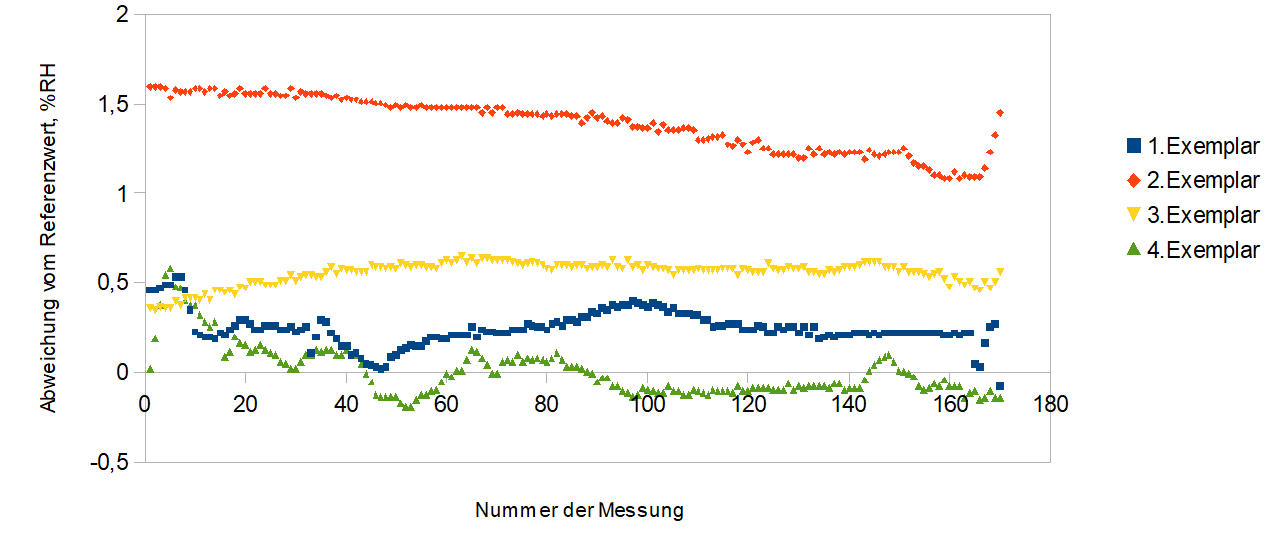
\includegraphics[width=\textwidth]{pictures/HTU21D_50.png}
\caption{HTU21DF Abweichung von Referenzwerten während der Messung bei 50\% RH}
% \label{fig1}
\end{figure}

\begin{figure}[h]
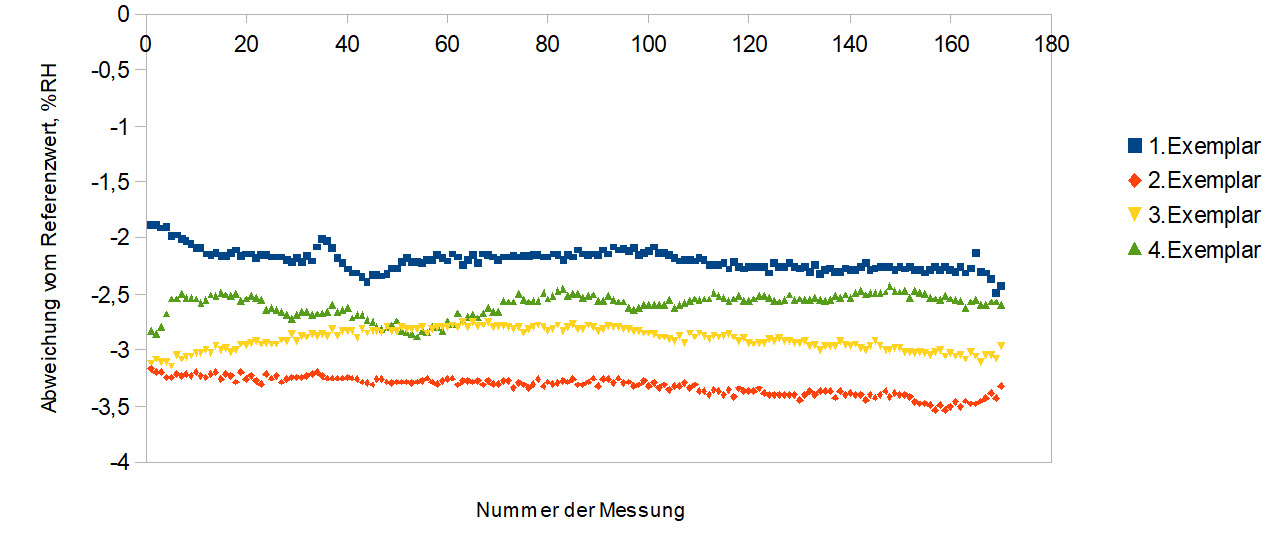
\includegraphics[width=\textwidth]{pictures/SHT31_50.png}
\caption{SHT31 Abweichung von Referenzwerten während der Messung bei 50\% RH}
% \label{fig1}
\end{figure}


\begin{figure}[h]
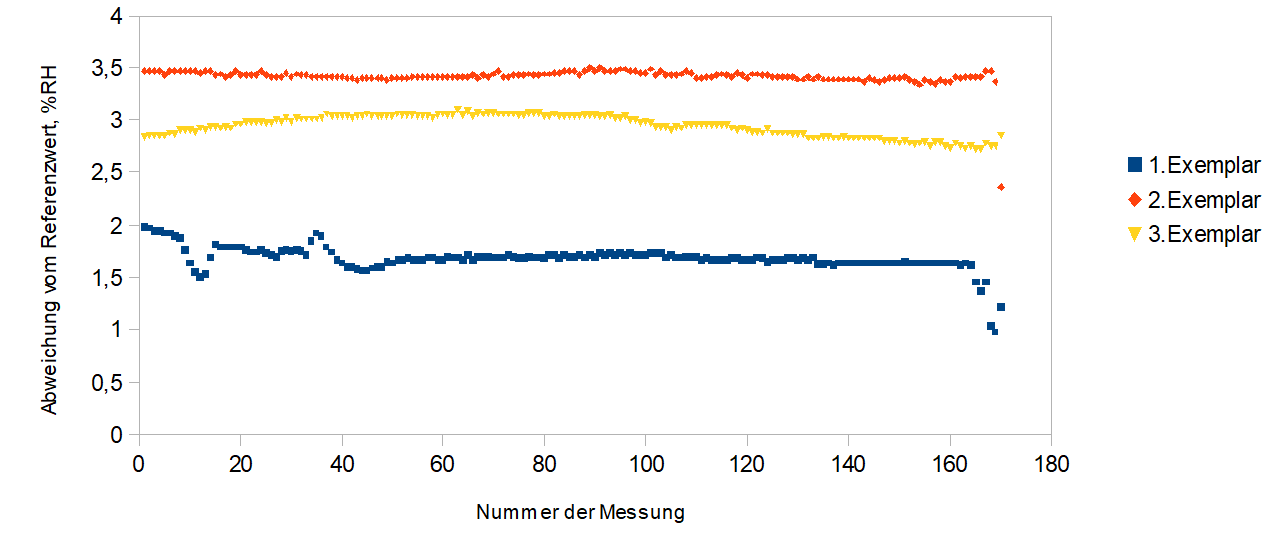
\includegraphics[width=\textwidth]{pictures/BME280_50.png}
\caption{BME280 Abweichung von Referenzwerten während der Messung bei 50\% RH}
% \label{fig1}
\end{figure}

\begin{figure}[h]
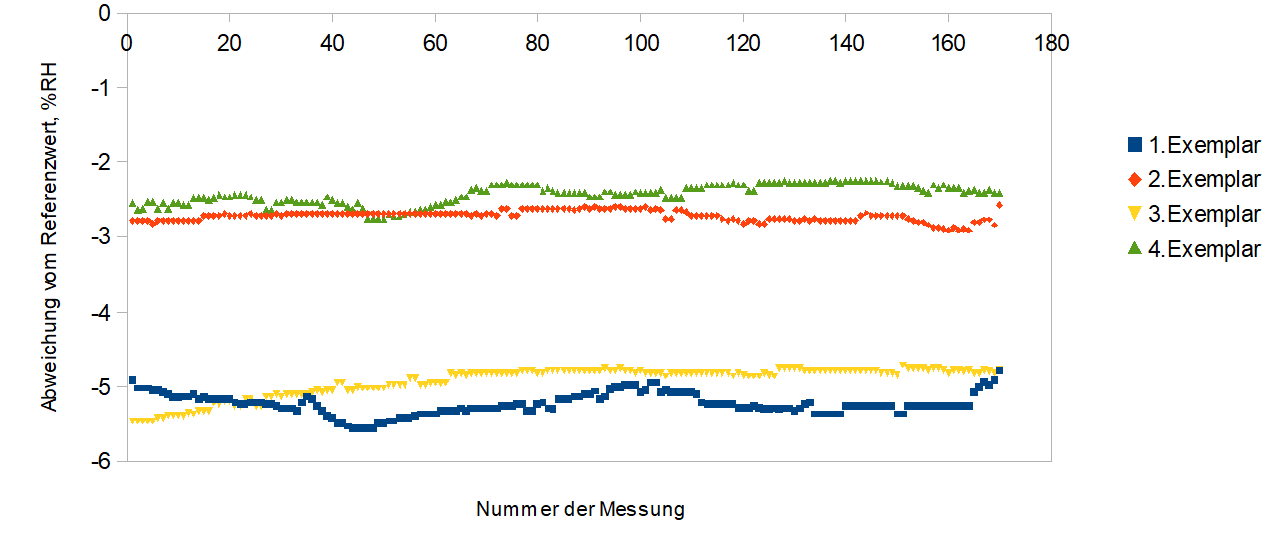
\includegraphics[width=\textwidth]{pictures/DHT22_50.png}
\caption{DHT22 Abweichung von Referenzwerten während der Messung bei 50\% RH}
% \label{fig1}
\end{figure}

\begin{figure}[h]
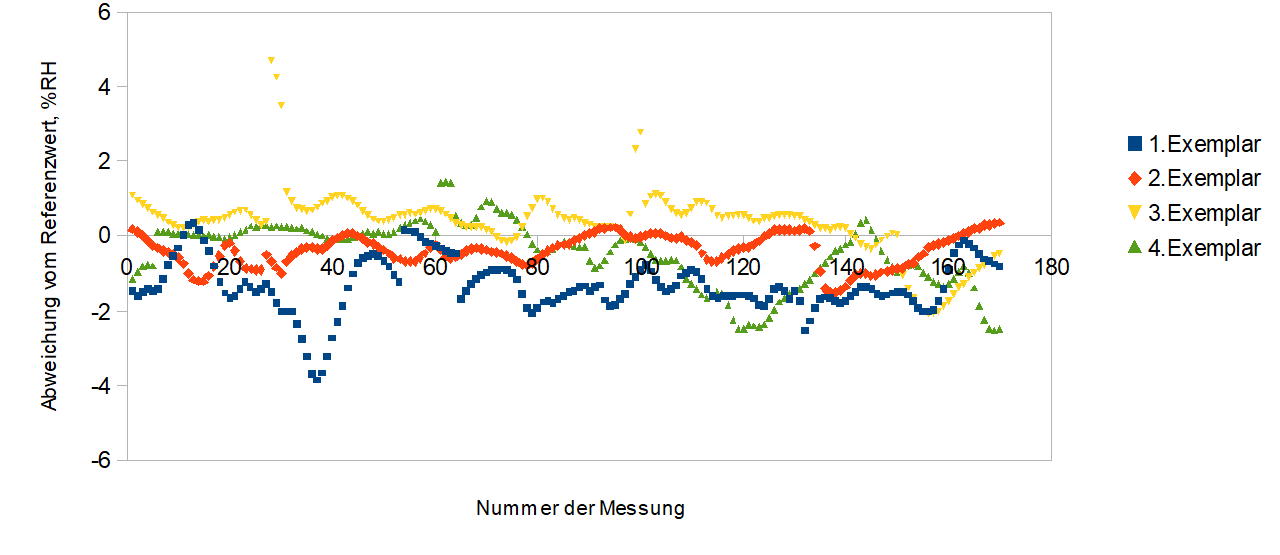
\includegraphics[width=\textwidth]{pictures/HTU21D_60.png}
\caption{HTU21DF Abweichung von Referenzwerten während der Messung bei 60\% RH}
% \label{fig1}
\end{figure}

\begin{figure}[h]
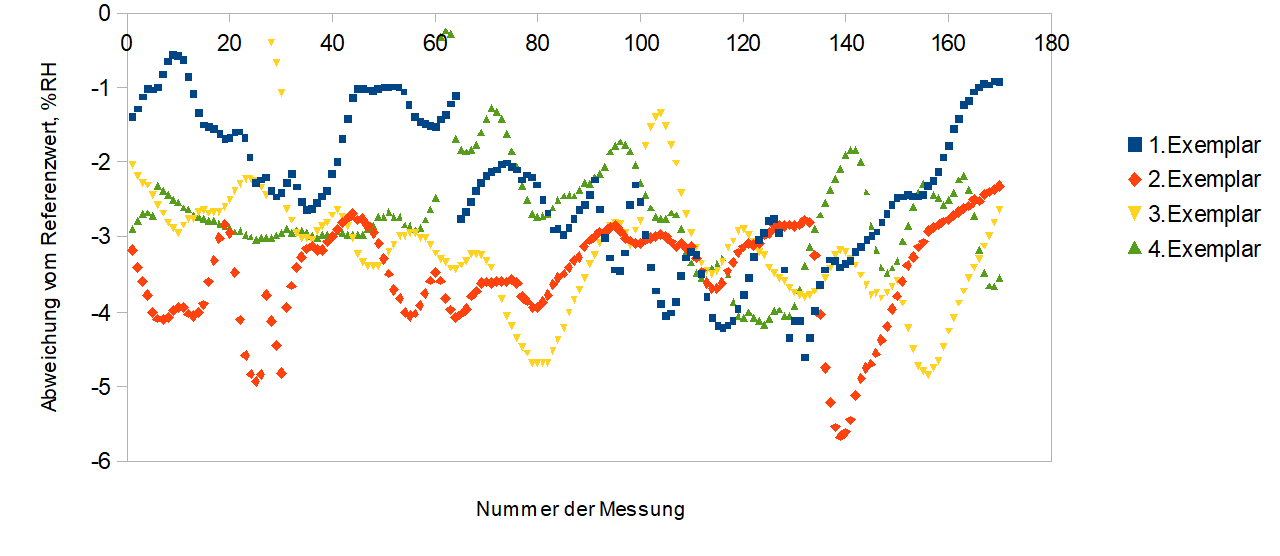
\includegraphics[width=\textwidth]{pictures/SHT31_60.png}
\caption{SHT31 Abweichung von Referenzwerten während der Messung bei 60\% RH}
% \label{fig1}
\end{figure}


\begin{figure}[h]
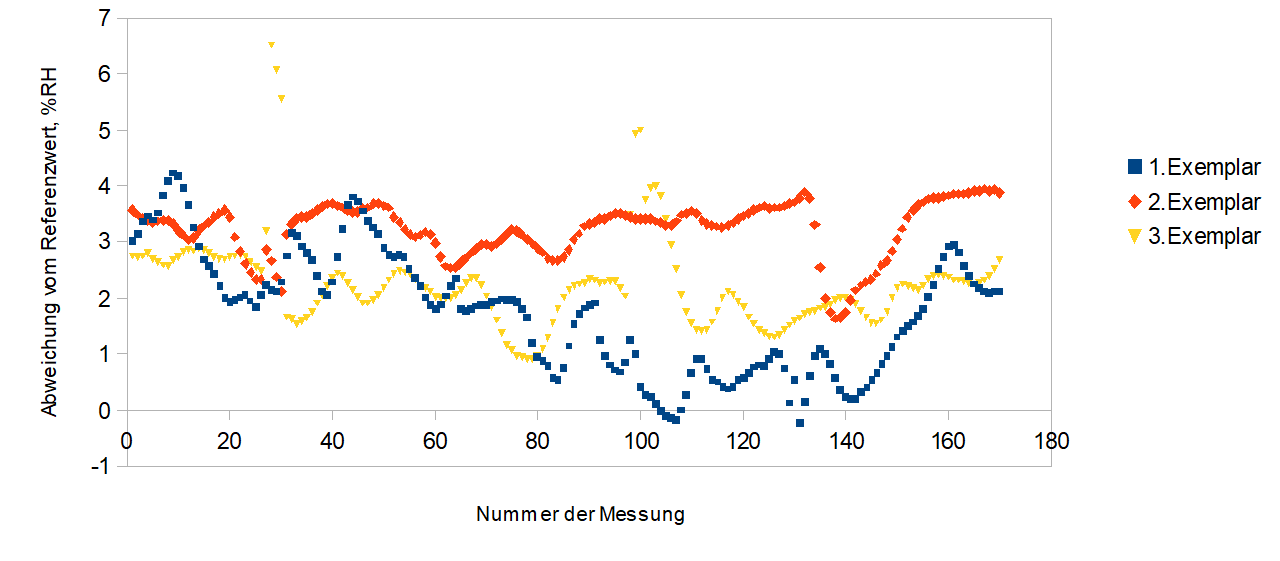
\includegraphics[width=\textwidth]{pictures/BME280_60.png}
\caption{BME280 Abweichung von Referenzwerten während der Messung bei 60\% RH}
% \label{fig1}
\end{figure}

\begin{figure}[h]
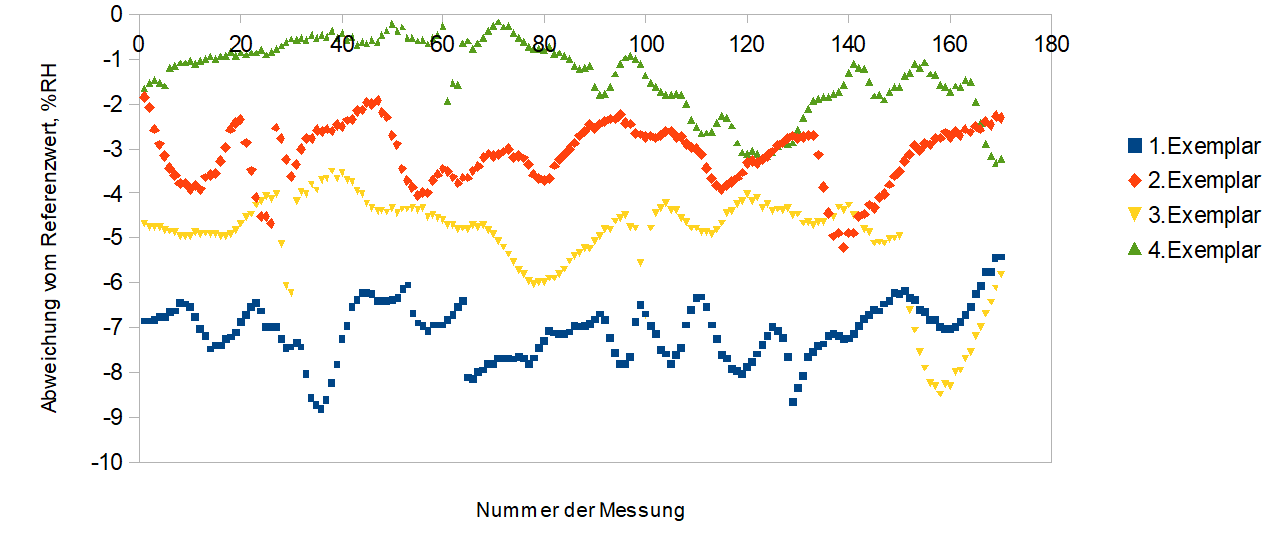
\includegraphics[width=\textwidth]{pictures/DHT22_60.png}
\caption{DHT22 Abweichung von Referenzwerten während der Messung bei 60\% RH}
% \label{fig1}
\end{figure}

\begin{figure}[h]
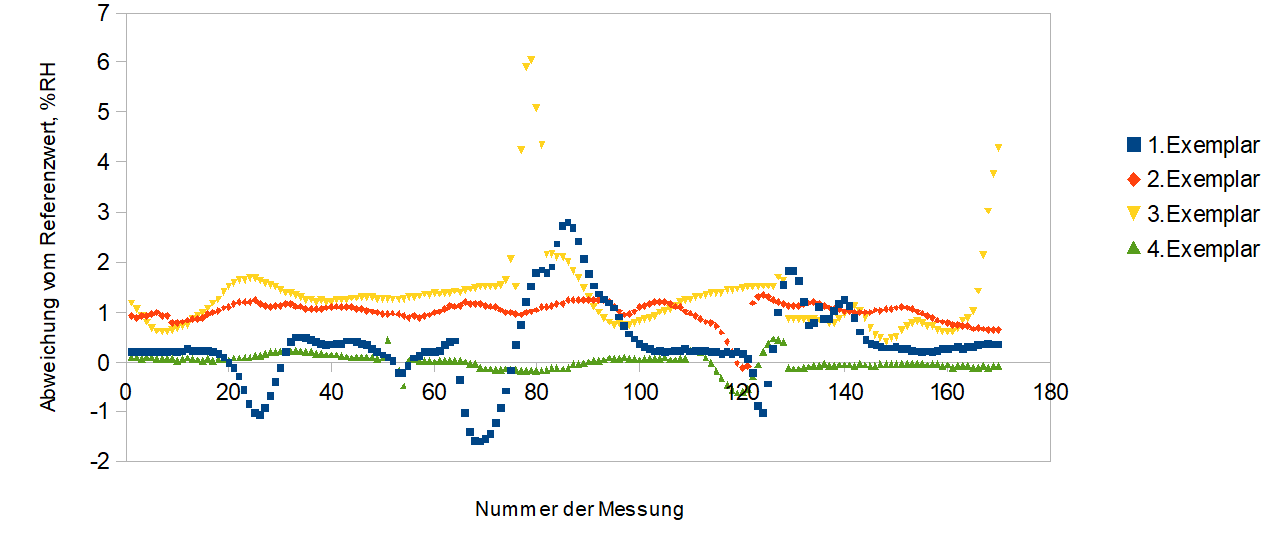
\includegraphics[width=\textwidth]{pictures/HTU21D_70.png}
\caption{HTU21DF Abweichung von Referenzwerten während der Messung bei 70\% RH}
% \label{fig1}
\end{figure}

\begin{figure}[h]
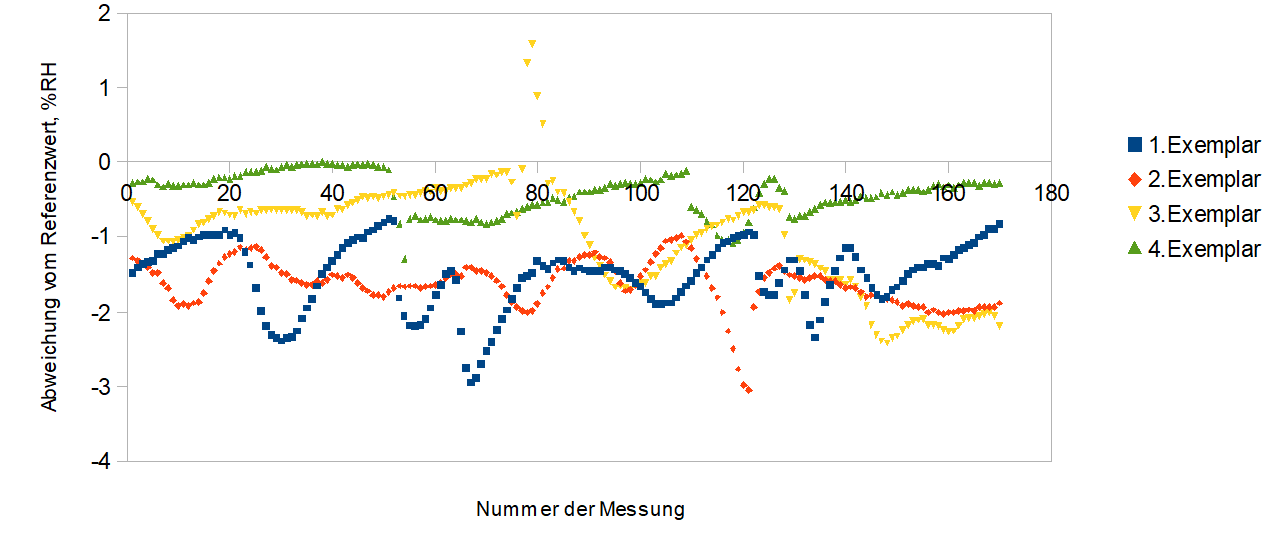
\includegraphics[width=\textwidth]{pictures/SHT31_70.png}
\caption{SHT31 Abweichung von Referenzwerten während der Messung bei 70\% RH}
% \label{fig1}
\end{figure}


\begin{figure}[h]
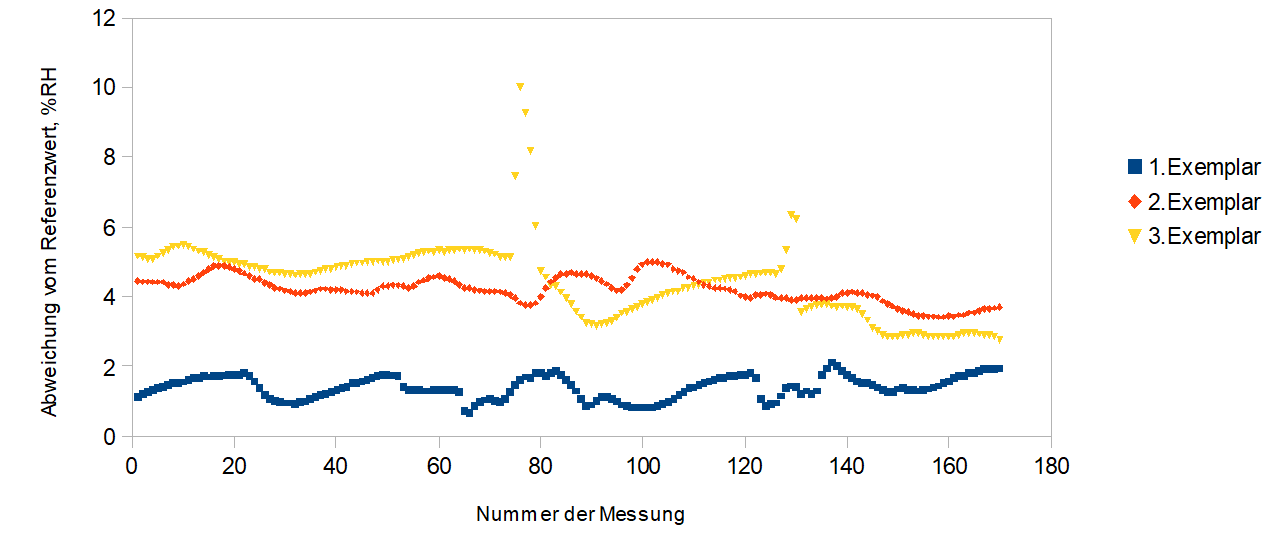
\includegraphics[width=\textwidth]{pictures/BME280_70.png}
\caption{BME280 Abweichung von Referenzwerten während der Messung bei 70\% RH}
% \label{fig1}
\end{figure}

\begin{figure}[h]
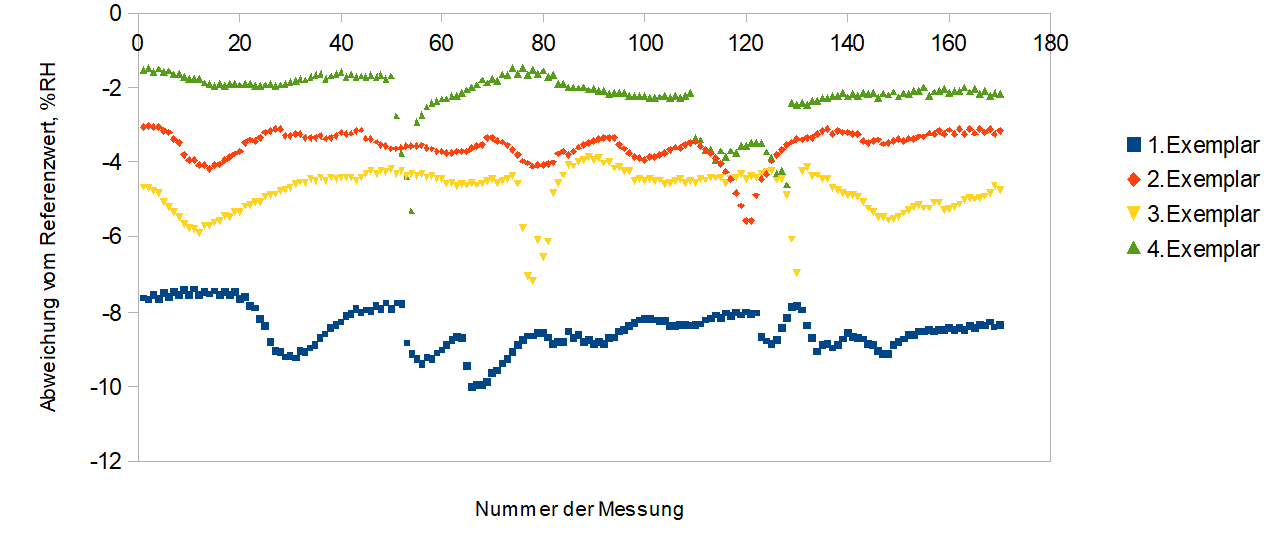
\includegraphics[width=\textwidth]{pictures/DHT22_70.png}
\caption{DHT22 Abweichung von Referenzwerten während der Messung bei 70\% RH}
% \label{fig1}
\end{figure}

\begin{figure}[h]
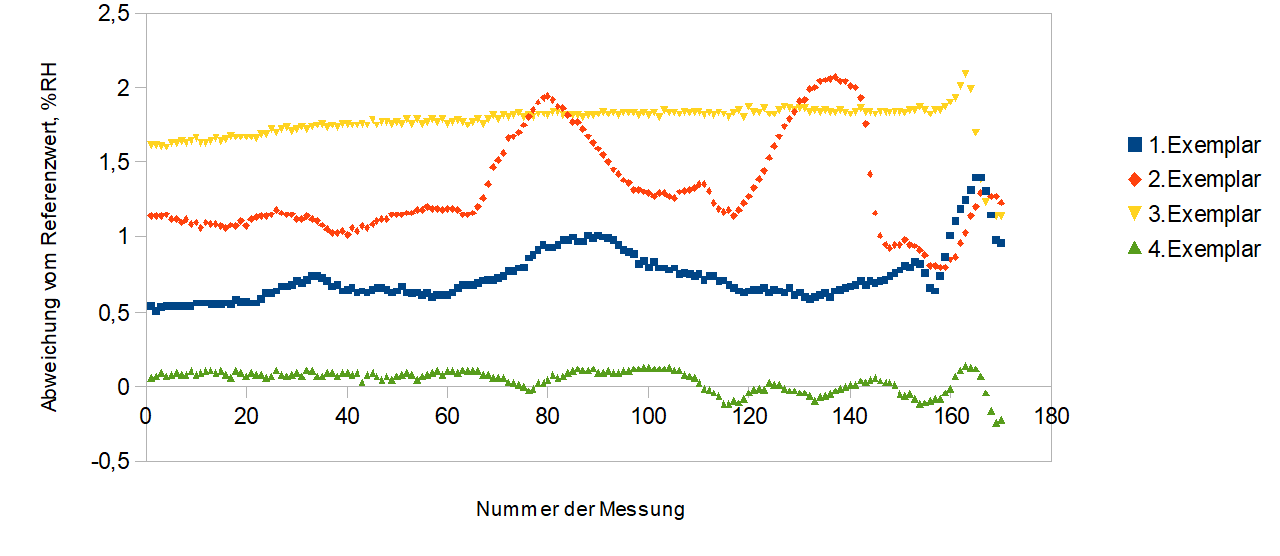
\includegraphics[width=\textwidth]{pictures/HTU21D_80.png}
\caption{HTU21DF Abweichung von Referenzwerten während der Messung bei 80\% RH}
% \label{fig1}
\end{figure}

\begin{figure}[h]
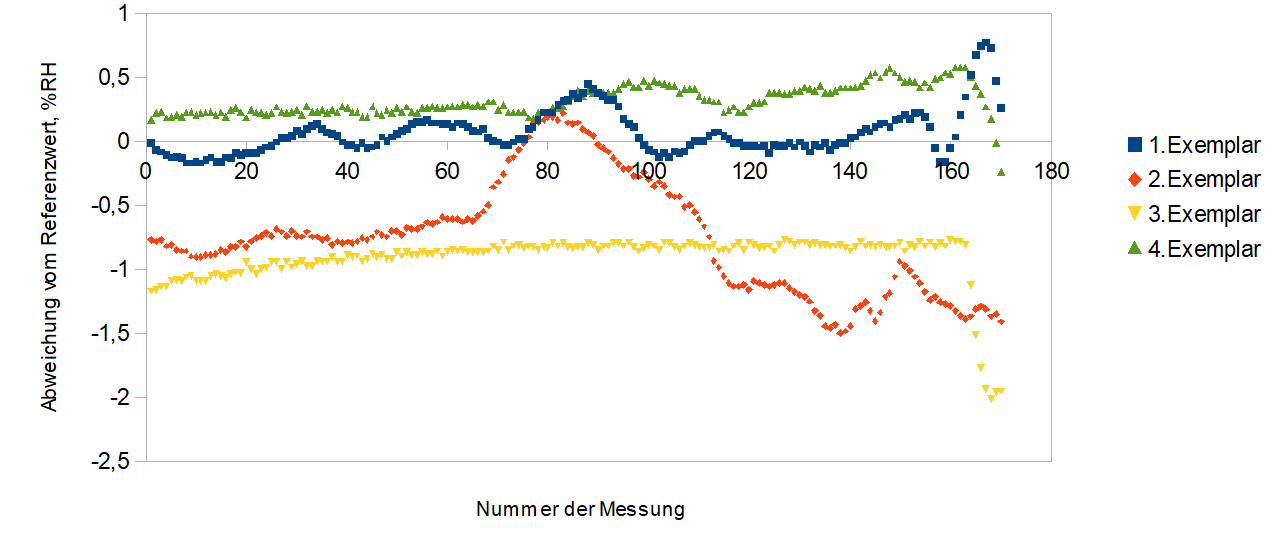
\includegraphics[width=\textwidth]{pictures/SHT31_80.png}
\caption{SHT31 Abweichung von Referenzwerten während der Messung bei 80\% RH}
% \label{fig1}
\end{figure}


\begin{figure}[h]
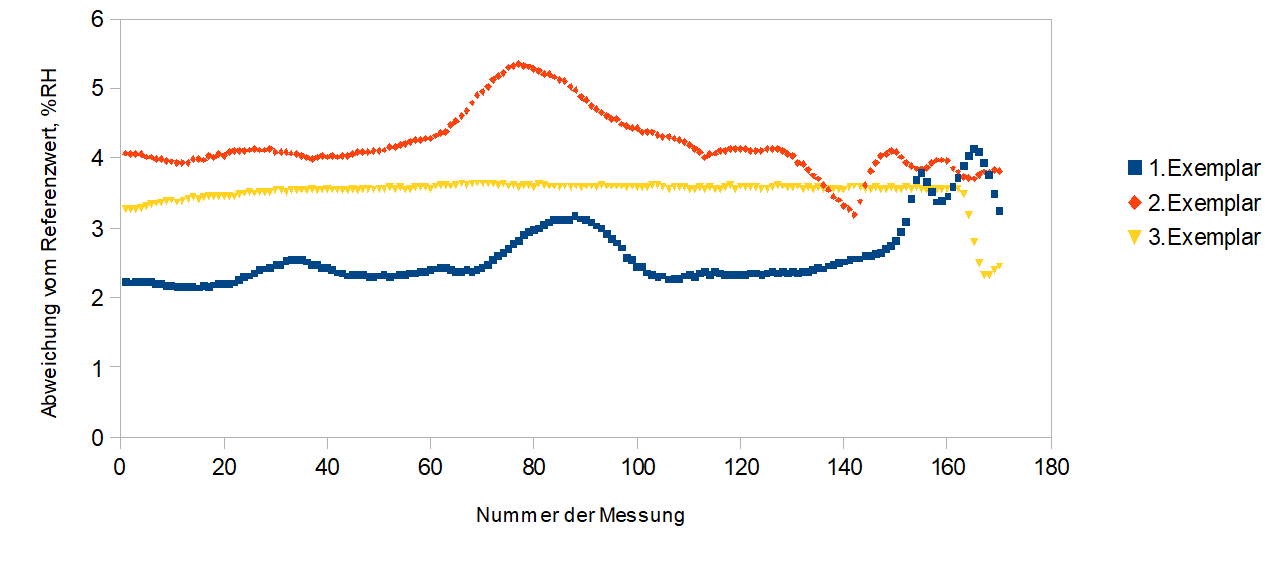
\includegraphics[width=\textwidth]{pictures/BME280_80.png}
\caption{BME280 Abweichung von Referenzwerten während der Messung bei 80\% RH}
% \label{fig1}
\end{figure}

\begin{figure}[h]
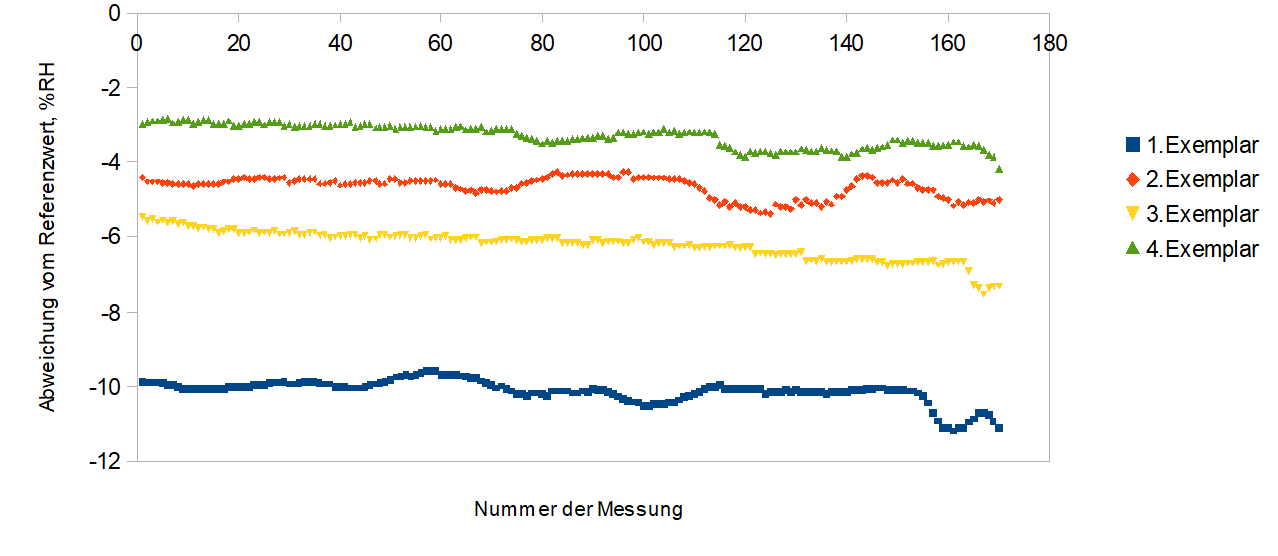
\includegraphics[width=\textwidth]{pictures/DHT22_80.png}
\caption{DHT22 Abweichung von Referenzwerten während der Messung bei 80\% RH}
% \label{fig1}
\end{figure}

\clearpage

\subsection{Programm}

\begin{lstlisting}[language=C]
#include "SD.h"
#include <Wire.h>
#include "Adafruit_HTU21DF.h"
#include "Adafruit_SHT31.h"
#include <Adafruit_BME280.h>
#include <Sensirion.h>
#include "DHT.h"
#include "FS.h"
#include "SPI.h"
#include "TimeLib.h"

#define SDA_SHT75 32
#define SCL_SHT75 33

#define SDA_HTU21 25
#define SCL_HTU21 26

#define SDA_SHT31 13
#define SCL_SHT31 14

#define SDA_BME280 21
#define SCL_BME280 22

#define SDA_DHT22 4
#define DHTTYPE DHT22

#define NUM_MEASUREMENTS 10

/*Temperatur, Feuchtigkeit, Zeit wann 
gemessen wurde * fuenf Sensoren 3*5 = 15*/
#define NUM_PARAMETERS 15 

#define DELAY_TIME 500
#define STRING_LENGTH 300


Sensirion sht75 = Sensirion(SDA_SHT75, SCL_SHT75);
float temperature_sht75;
float humidity_sht75;
float dewpoint_sht75;

Adafruit_HTU21DF htu21 = Adafruit_HTU21DF();

Adafruit_SHT31 sht31 = Adafruit_SHT31();

Adafruit_BME280 bme280 = Adafruit_BME280();
TwoWire wire_bme280 = TwoWire(5);

DHT dht22(SDA_DHT22, DHTTYPE);

/*measurements[x][y]:
  x ist i-te Messung
  y=0 Temp.   SHT75
  y=1 Feucht. SHT75
  y=2 die seit dem Einschalten des Mikrokontrollers vergangene Zeit
      in Millisekunden SHT75
  y=3 Temp.   HTU21
  y=4 Feucht. HTU21
  y=5 die seit dem Einschalten des Mikrokontrollers vergangene Zeit
      in Millisekunden HTU21 
  y=6 Temp.   SHT31
  y=7 Feucht. SHT31
  y=8 die seit dem Einschalten des Mikrokontrollers vergangene Zeit
      in Millisekunden SHT31
  y=9 Temp.   BME280
  y=10 Feucht.BME280
  y=11 die seit dem Einschalten des Mikrokontrollers vergangene Zeit
       in Millisekunden BME280
  y=12 Temp.  DHT22
  y=13 Feucht.DHT22
  y=14 die seit dem Einschalten des Mikrokontrollers vergangene Zeit
       in Millisekunden DHT22
*/
float measurements[NUM_MEASUREMENTS][NUM_PARAMETERS];

int counter = 0;
int totalMeasurementCounter = 0;
char fileName[32];


void doMeasurement() {
  
  sht75.measure(&measurements[counter][0], &measurements[counter][1],
                &dewpoint_sht75);
  measurements[counter][2] = (float)millis();
  
  htu21.begin(SDA_HTU21, SCL_HTU21);
  measurements[counter][3] = htu21.readTemperature();
  measurements[counter][4] = htu21.readHumidity();
  measurements[counter][5] =  (float)millis();
  
  sht31.begin(SDA_SHT31, SCL_SHT31);
  measurements[counter][6] = sht31.readTemperature();
  measurements[counter][7] = sht31.readHumidity();
  measurements[counter][8] =  (float)millis();

  measurements[counter][9] = bme280.readTemperature();
  measurements[counter][10] = bme280.readHumidity();
  measurements[counter][11] = (float)millis();

  measurements[counter][12] = dht22.readTemperature();
  measurements[counter][13] = dht22.readHumidity();
  measurements[counter][14] =  (float)millis();
  
}

void printLastMeasurement() {
  
  Serial.print("SHT75 Temp: "); Serial.print(measurements[counter][0]);
  Serial.print("; Hum: "); Serial.print(measurements[counter][1]);
  Serial.print("; Time: "); Serial.println(measurements[counter][2]);
  
  Serial.print("HTU21DF Temp: "); Serial.print(measurements[counter][3]);
  Serial.print("; Hum: "); Serial.print(measurements[counter][4]);
  Serial.print("; Time: "); Serial.println(measurements[counter][5]);
  
  Serial.print("SHT31 Temp: "); Serial.print(measurements[counter][6]);
  Serial.print("; Hum: "); Serial.print(measurements[counter][7]);
  Serial.print("; Time: "); Serial.println(measurements[counter][8]);
  
  Serial.print("BME280 Temp: "); Serial.print(measurements[counter][9]);
  Serial.print("; Hum: "); Serial.print(measurements[counter][10]);
  Serial.print("; Time: "); Serial.println(measurements[counter][11]);

  Serial.print("DHT22 Temp: "); Serial.print(measurements[counter][12]);
  Serial.print("; Hum: "); Serial.print(measurements[counter][13]);
  Serial.print("; Time: "); Serial.println(measurements[counter][14]);
  Serial.println("");

}

void writeMeasurementsOnSdCard() {
  char buffer[NUM_MEASUREMENTS][STRING_LENGTH];
  for(int i = 0; i < NUM_MEASUREMENTS; i++) {
    String measurement = String(totalMeasurementCounter) + ";"
                       + String(measurements[i][0]) + ";" 
                       + String(measurements[i][1]) + ";" 
                       + String(measurements[i][2])
                       + ";" + String(measurements[i][3]) 
                       + ";" + String(measurements[i][4]) 
                       + ";" + String(measurements[i][5])
                       + ";" + String(measurements[i][6]) 
                       + ";" + String(measurements[i][7]) 
                       + ";" + String(measurements[i][8])
                       + ";" + String(measurements[i][9]) + ";" 
                       + String(measurements[i][10]) + ";" 
                       + String(measurements[i][11])
                       + ";" + String(measurements[i][12]) 
                       + ";" + String(measurements[i][13]) + ";" 
                       + String(measurements[i][14]); 
                 
    
    measurement.toCharArray(buffer[i],STRING_LENGTH);
    totalMeasurementCounter++;
  }
  appendFile(SD, fileName, buffer);
}


void createFileName(fs::FS &fs) {
  String fileNameStr = "/measurements_";
  char fileNameChar[32];
  int numOfFiles = 0;
  File dir = fs.open("/");
  while(dir.openNextFile()) {
    numOfFiles++;
  }
  fileNameStr = fileNameStr + String(numOfFiles) + ".txt";
  fileNameStr.toCharArray(fileName,32);
  Serial.print("Created name: ");
  Serial.println(fileName);
}

void writeFile(fs::FS &fs, const char * message){
    createFileName(fs);
    Serial.printf("Writing file: %s\n", fileName);
    File file = fs.open(fileName, FILE_WRITE);
    if(!file){
        Serial.println("Failed to open file for writing");
        return;
    }
    if(file.print(message)){
        Serial.println("File written");
    } else {
        Serial.println("Write failed");
    }
    file.close();
}

void appendFile(fs::FS &fs, const char * path, 
                char messages[NUM_MEASUREMENTS][STRING_LENGTH]){
    Serial.printf("Appending to file: %s\n", path);

    File file = fs.open(path, FILE_APPEND);
    if(!file){
        Serial.println("Failed to open file for appending");
        return;
    }
    for(int i = 0; i < NUM_MEASUREMENTS; i++) {
      if(file.println(messages[i])){
          Serial.println("Message appended");
      } else {
          Serial.println("Append failed");
      }
    }

    file.close();
}


void setup() {
  Serial.begin(9600);
  Serial.println("Beginning");
  
  dht22.begin();
  
  wire_bme280.begin(SDA_BME280,SCL_BME280);
  bme280.begin(&wire_bme280); 

  if(!SD.begin()){
      Serial.println("Card Mount Failed");
      return;
  }
  uint8_t cardType = SD.cardType();

  if(cardType == CARD_NONE){
      Serial.println("No SD card attached");
      return;
  }

  Serial.print("SD Card Type: ");
  if(cardType == CARD_MMC){
      Serial.println("MMC");
  } else if(cardType == CARD_SD){
      Serial.println("SDSC");
  } else if(cardType == CARD_SDHC){
      Serial.println("SDHC");
  } else {
      Serial.println("UNKNOWN");
  }

  uint64_t cardSize = SD.cardSize() / (1024 * 1024);
  Serial.printf("SD Card Size: %lluMB\n", cardSize);

  Serial.printf("Total space: %lluMB\n", SD.totalBytes() / (1024 * 1024));
  Serial.printf("Used space: %lluMB\n", SD.usedBytes() / (1024 * 1024));
  writeFile(SD, 
   "Meas_numb;SHT75_temp;SHT75_hum;SHT75_time;
   HTU21DF_temp;HTU21DF_hum;HTU21DF_time;
   SHT31_temp;SHT31_hum;SHT31_time;
   BME280_temp;BME280_hum;BME280_time;DHT22_temp;
   DHT22_hum;DHT22_time\n");

}


void loop() {
  if(counter == NUM_MEASUREMENTS) {
    writeMeasurementsOnSdCard();
    counter = 0;
  }
  doMeasurement();
  printLastMeasurement();
  counter++;
  delay(DELAY_TIME);
}

\end{lstlisting}
\end{document}
